
\documentclass{article}
\usepackage[headheight=20pt, margin=1.0in, top=1.2in]{geometry}
\usepackage{amsmath, amssymb, amsthm, thmtools, tcolorbox, array, graphicx, makeidx, cancel, multirow, fancyhdr, xypic, color, nicefrac, rotating, multicol, caption, subcaption, xcolor, tikz, tikz-3dplot, tikz-cd, pgfplots, import, enumitem, calc, booktabs, wrapfig, siunitx, hyperref,float}
\hypersetup{colorlinks=true,linkcolor=blue}
\usepackage[all]{xy}
\usepackage{esint}
\setlength{\parindent}{0in}
\sisetup{per-mode = symbol}
\usetikzlibrary{calc,arrows,svg.path,decorations.markings,patterns,matrix,3d,fit}
\usepgfplotslibrary{groupplots}
\pgfplotsset{compat=newest}
\newtcolorbox{mydefbox}[2][]{colback=red!5!white,colframe=red!75!black,fonttitle=\bfseries,title=#2,#1}
\newtcolorbox{mythmbox}[2][]{colback=gray!5!white,colframe=gray!75!black,fonttitle=\bfseries,title=#2,#1}
\newtcolorbox{myexamplebox}[2][]{colback=green!5!white,colframe=green!75!black,fonttitle=\bfseries,title=#2,#1}
\newtcolorbox{mypropbox}[2][]{colback=blue!5!white,colframe=blue!75!black,fonttitle=\bfseries,title=#2,#1}
\declaretheoremstyle[headfont=\color{blue}\normalfont\bfseries,]{colored}
\theoremstyle{definition}
\newtheorem{theorem}{Theorem}
\newtheorem{corollary}[theorem]{Corollary}
\newtheorem{lemma}[theorem]{Lemma}
\newtheorem{proposition}[theorem]{Proposition}
\newtheorem{problem}[theorem]{Problem}
\newtheorem{definition}[theorem]{Definition}
\newtheorem{exercise}[theorem]{Exercise}
\newtheorem{example}[theorem]{Example}
\newtheorem{solution}[theorem]{Solution}
\newtheorem*{thm}{Theorem}
\newtheorem*{lem}{Lemma}
\newtheorem*{prob}{Problem}
\newtheorem*{exer}{Exercise}
\newtheorem*{prop}{Proposition}
\def\R{\mathbb{R}}
\def\F{\mathbb{F}}
\def\Q{\mathbb{Q}}
\def\C{\mathbb{C}}
\def\N{\mathbb{N}}
\def\Z{\mathbb{Z}}
\def\Ra{\Rightarrow}
\def\e{\epsilon}
\newcommand{\typo}[1]{{\color{red}{#1}}}
\newcommand\thedate{\today}
\newcommand{\mb}{\textbf}
\newcommand{\norm}[2]{\|{#1}\|_{#2}}
\newcommand{\normm}[1]{\|#1\|}
\newcommand{\mat}[1]{\begin{bmatrix} #1 \end{bmatrix}}
\newcommand{\eqtext}[1]{\hspace{3mm} \text{#1} \hspace{3mm}}
\newcommand{\set}[1]{\{#1\}}
\newcommand{\inte}{\textrm{int}}
\newcommand{\ra}{\rightarrow}
\newcommand{\minv}{^{-1}}
\newcommand{\tx}[1]{\text{ {#1} }}
\newcommand{\abs}[1]{|#1|}
\newcommand{\mc}[1]{\mathcal{#1}}
\newcommand{\uniflim}{\mathop{\mathrm{unif\lim}}}
\newcommand{\notimplies}{\mathrel{{\ooalign{\hidewidth$\not\phantom{=}$\hidewidth\cr$\implies$}}}}
\pagestyle{fancy}
\fancyhf{}
\fancyhead[L]{Title of the Document}
\fancyhead[C]{}
\fancyhead[R]{\thepage}
\fancyfoot[L]{}
\fancyfoot[C]{}
\fancyfoot[R]{}
\renewcommand{\headrulewidth}{0.4pt}
\renewcommand{\footrulewidth}{0.4pt}
\numberwithin{equation}{section}
% Increase spacing between paragraphs
\setlength{\parskip}{1em}
% Increase spacing before and after sections
\usepackage{titlesec}
\titlespacing*{\section}{0pt}{3ex plus 1ex minus .2ex}{2ex plus .2ex}
\titlespacing*{\subsection}{0pt}{2ex plus 1ex minus .2ex}{1ex plus .2ex}
\titlespacing*{\subsubsection}{0pt}{1ex plus 1ex minus .2ex}{1ex plus .2ex}
\title{\textbf{Title of the Document}}
\author{Author Name}
\date{\today}
\begin{document}
\maketitle
\tableofcontents
\newpage
\section{Exercises}
\textbf{2-1.} Let $(X,d)$ be a metric space and $S \subset X$. Show that $\overline{S} = S^*$ iff $S = \overline{S} \cap S^{int} = \emptyset$. \\
\textbf{2-2.} Show that for an arbitrary choice of $a,b,c \in \mathbb{R}$, the closed disk $(x - a)^2 + (y - b)^2 \leq r^2$ is a bounded set in $\mathbb{R}^2$. \\
\textbf{2-3.} Let $(X, d)$ be a metric space and for $x,y \in X$. Show that if $d(x, y) < \varepsilon$ for every $\varepsilon > 0$, then $x = y$.

\begin{proof}[Solution 2-1]
Assume $S \neq \overline{S} \cap S^{int}$. \\
Then $\exists x \in S^{int} : x \in \overline{S} \cap x \notin S^{int}$. \\
Then by $x \in S^{int} \Rightarrow \exists \varepsilon > 0 : B_{\varepsilon}(x) \subseteq S^1$. \\
However, by $x \notin S^{int}$, this value of $\varepsilon > 0$ implies 
$ 
B_{\frac{\varepsilon}{4}}(x) \cap S^1 = \emptyset \Rightarrow B_{\frac{\varepsilon}{4}}(x) \nsubseteq S,
$
which is a contradiction, implying our assumption that $x \in \overline{S} \cap S^{int}$ must be false and 
$ 
\overline{S} \cap S^{int} = \emptyset.
$
\end{proof}

\begin{proof}[Solution 2-2]
A set $S$ is bounded iff $\exists M \in \mathbb{R}^+ : \forall x,y \in S$.
$ 
d(x,y) \leq M.
$

Let $a,b,r \in \mathbb{R}$.
$
S:= \{(x,y) \in \mathbb{R}^2  |(x - a)^2 + (y - b)^2 \leq r^2\}
$
$
\Rightarrow x^2 - 2ax + a^2 + y^2 - 2yb + b^2 \leq r^2 
$
$
\Rightarrow x^2 - 2ax + y^2 - 2yb \leq r^2 - a^2 - b^2
$
$
\Rightarrow x^2 + y^2 \leq r^2 - a^2 - b^2 + 2ax + 2yb
$

Need to show $x^2$ is bounded:
$
(x - a)^2 \leq r^2
$
$
\Rightarrow |x - a| \leq |r| 
$
$
\Rightarrow |x - a| \leq |r| + |a| 
$
$
\Rightarrow |x| = |x - a + a| \leq |x - a| + |a| \leq r + |a|.
$

\end{proof}

\begin{align*}
&\implies |y| \leq r + |a| \\
&\implies x^2 \leq (r + |a|)^2
\end{align*}

\text{Same for } y: \quad y^2 \leq (r + |b|)^2

\begin{align*}
&\forall z = (x, y) \in D_{r, a, b}, \\
&\|z\| = \sqrt{x^2 + y^2} \\
&\leq \sqrt{(r + |a|)^2 + (r + |b|)^2}
\end{align*}

Thus, if \(\mathcal{M} = \sqrt{(r + |a|)^2 + (r + |b|)^2}\), the bound holds.

\#1S \text{ normed boundedness = distance boundedness.}

Let \( x = (x_1, x_2), \, y = (y_1, y_2) \in \mathbb{P}_{r, a, b} \)

\begin{align*}
z_1 &= (x, y) \\
(z_1 - a)^2 + (z_2 - b)^2 &= r^2 \\
\Rightarrow d(z, (a, b)) &= \sqrt{(z_1 - a)^2 + (z_2 - b)^2} \leq r \\
\Rightarrow d(x, y) &\leq d(x, (a, b)) + d(y, (a, b)) \\
&= \sqrt{(x_1 - a)^2 + (x_2 - b)^2} + \sqrt{(y_1 - a)^2 + (y_2 - b)^2} \\
&\leq r + r = 2r.
\end{align*}

\section*{(iii)}
Suppose that \( x \neq y \). Then \( d(x, y) \neq 0 \). Thus if we choose \( \varepsilon = d(x, y) \) \(\implies \varepsilon > 0 \) but \( d(x, y) \in \varepsilon \). (contradiction).

\textbf{(contradiction)} Suppose \( x \neq y \) and so \( d(x, y) \neq 0 \).

Choose \( \varepsilon > 0 \) so that \( \varepsilon = d(x, y) \). Then we must have \( d(x, y) < \varepsilon = d\left(\frac{\varepsilon}{2}\right) \), which is a contradiction, as this implies \( d(x, y) = \frac{\varepsilon}{2} \).

Thus \( d(x, y) \leq 0\) \(\implies d(x, y) = 0\) \(\varepsilon = d(x, y) = \frac{\varepsilon}{2}\) \(\implies x = y \).

$
\varepsilon > \frac{\varepsilon}{2} \quad \implies 2s < \varepsilon
$

Thus \( x = y \).

\section*{(iv)}

Let \( (V, \| \cdot \|) \) be a normed vsp.

Then let \( r > 0 \) and \( x \in V \). Then

$
B_{r}(x) = \{ v \in V | d(x, v) < r \}
$
$
B_{\| x \| + r}(0) = \{ v \in V | d(0, v) < r + \| x \| \}
$

\textbf{Diagram:}
% Diagram of balls in a normed space
\begin{center}
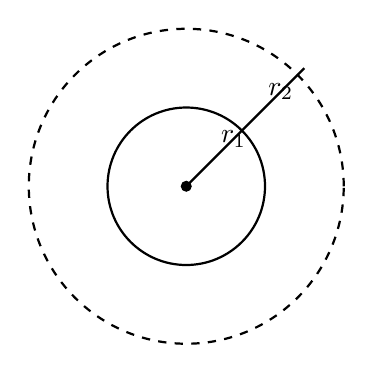
\begin{tikzpicture}
\draw[thick] (0,0) circle (1);
\draw[thick, dashed] (0,0) circle (2);
\fill (0,0) circle (2pt);
\draw[thick] (0,0) -- (1.5,1.5);
\node at (0.6,0.6) {$r_{1}$};
\node at (1.2,1.2) {$r_{2}$};
\end{tikzpicture}
\end{center}

Let \( y \in B_r (x) \).

$
d(0, y) \leq d(0, x) + d(x, y)
$
$
\leq \| x \| + r
$

\(\implies B_r (x) \subseteq B_{r + \| x \|} (0) \).

\section*{(v)}
Suppose \( S \) is bounded. Then \(\exists M \in \mathbb{R} : \forall x \in S \| x \| \leq M \).

$
\text{(Equiv to } \exists M \in \mathbb{R} \text{ :} \forall x \in S \subseteq V\) \((x \in B_M (0))
$\end{document}